\section{The Anonymous Face Tracking Panda}
As previously stated, living with a mental illness can be isolating and the stigma around mental health issues makes people hesitant to seek professional help. The primary purpose of this thesis is to create a functional prototype capable of connecting people with mental health specialists anonymously, while still maintaining client-therapist empathy.

\subsection{Approach}
A working prototype was developed using Unreal Engine Blueprints (a node-based interface to create gameplay elements), the UE4, Metahumans, and Live Link connected to an iPhone's camera. In the prototype, patients can communicate with mental health specialists via video conferencing anonymously, as patient's smartphone functions as a virtual camera that allows the mental health practitioner to see the patient's facial expressions in real-time via a virtual avatar.

Using an Apple device with the TrueDepth sensor and the Live Link Face app, one can capture numerous facial tracking points by creating a depth map of ones’ face while projecting and analyzing over 30,000 invisible dots, as well as capturing an infrared face image. The data collected by the Apple device and app is delivered to the UE4 environment via a directed internet connection maintained between the user's iPhone/iPad and the Unreal Engine. When data is received by Unreal Engine 4, it is evaluated and turned into VA movements via Live Link Plugin, as shown in Figure 1 and Figure 2.

\begin{figure}[h!]
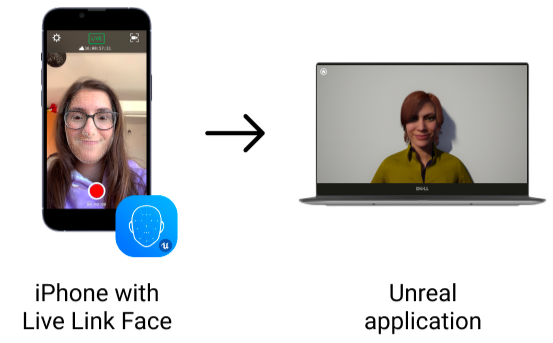
\includegraphics[width=0.7\textwidth]{figures/howItWorks.png}
\centering
\caption{How the facial expressions are captured and represented}
\end{figure}

\begin{figure}[h!]
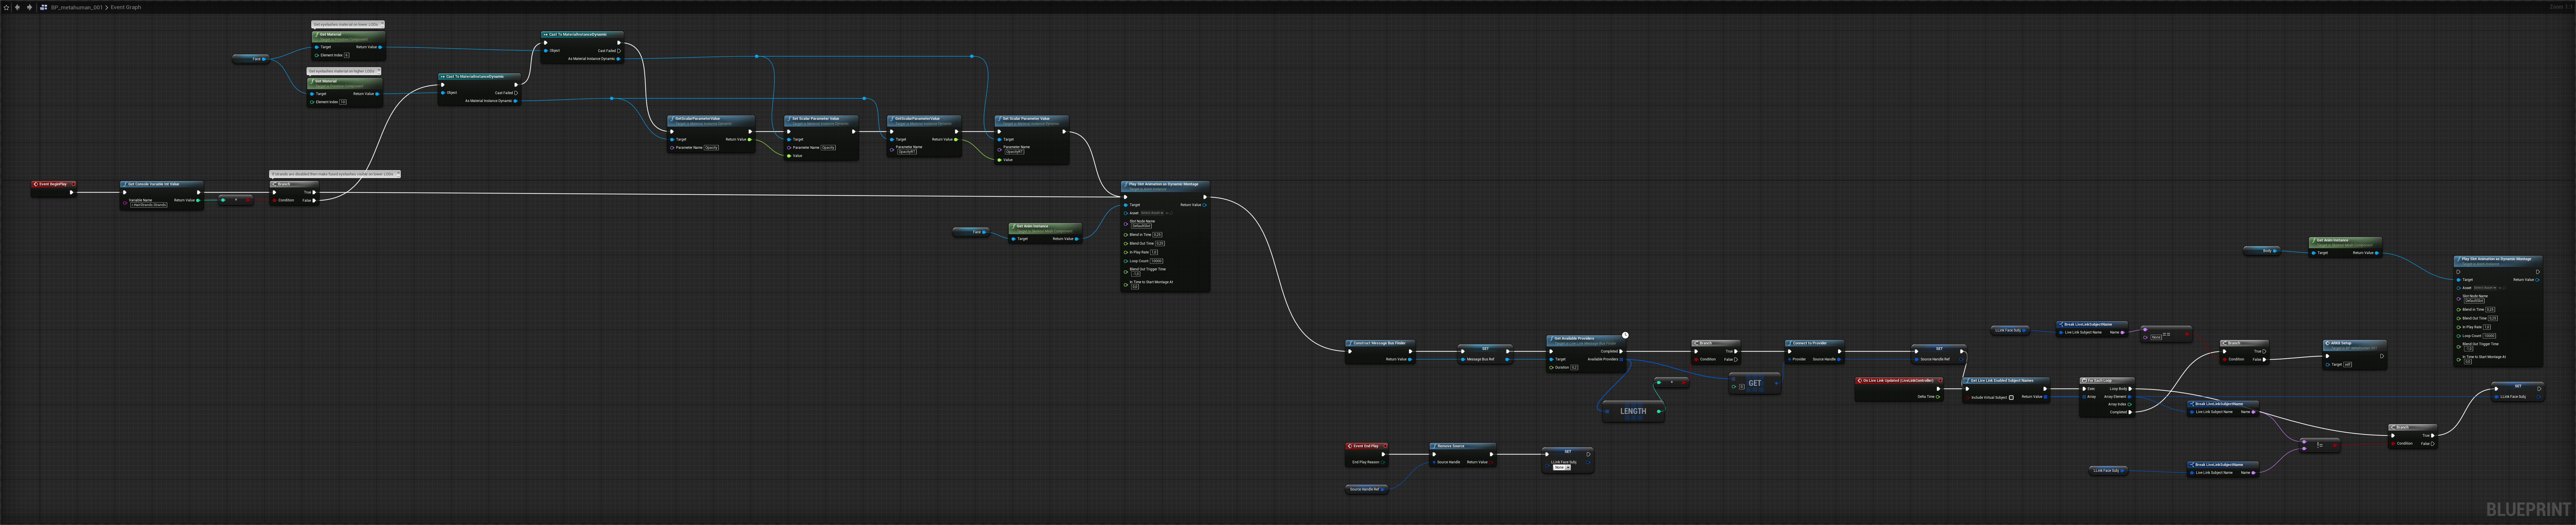
\includegraphics[width=\textwidth]{figures/hereItBegins.png}
\centering
\caption{Blueprints responsible for the connection and stream of data}
\end{figure}

The goal of the Live Link Plugin \cite{EPI22} is to provide a unified interface for streaming and consuming animation data into Unreal Engine 4 from one or more external sources, such as Display Data Channel (DDC) tools or Mocap Servers. It's built to be extensible via Unreal Plugins, allowing third parties to create new features without having to make and maintain Engine changes. Live Link can also be used by Motion Capture Systems to stream data into the Engine that can be previewed in real time.

To provide users with options, and thus reach a wider audience, four metahumans (two males and two females, of different ethnicities) were exported from the Metahuman Creator \cite{EPI21}, and the Quixel Bridge application into UE4, where, in order to make the interaction with the prototype easier, a minimalist user interface (Figure 4) was created that allows users to choose their preferred avatar. 

Although custom metahumans were not employed in this version of the prototype, due to performance and optimization concerns, the chosen metahumans (Figure 3) were pre-made by Epic Games and available on Quixel Bridge. These concerns were alleviated by using these four metahumans because Epic Games pre-defines export settings and assets compatible with many devices.

\begin{figure}[h!]
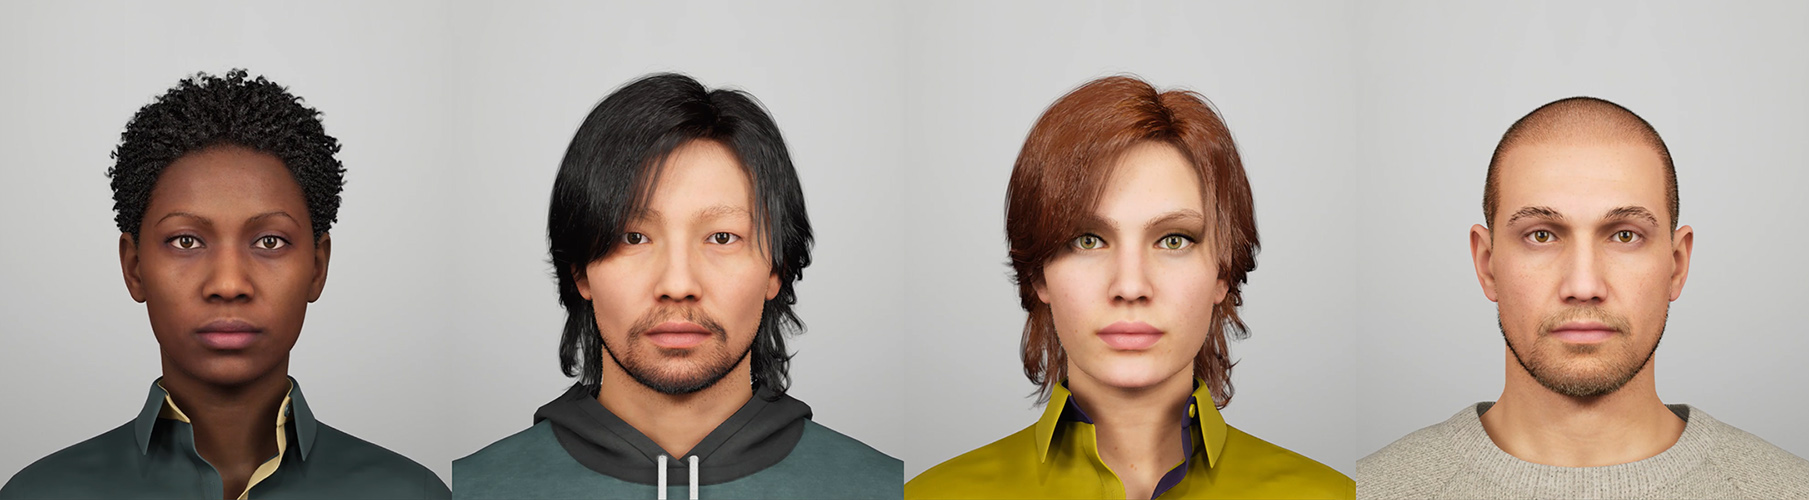
\includegraphics[width=\textwidth]{figures/4metahumans.jpg}
\centering
\caption{The current metahumans used on the prototype}
\end{figure}


\begin{figure}[h!]
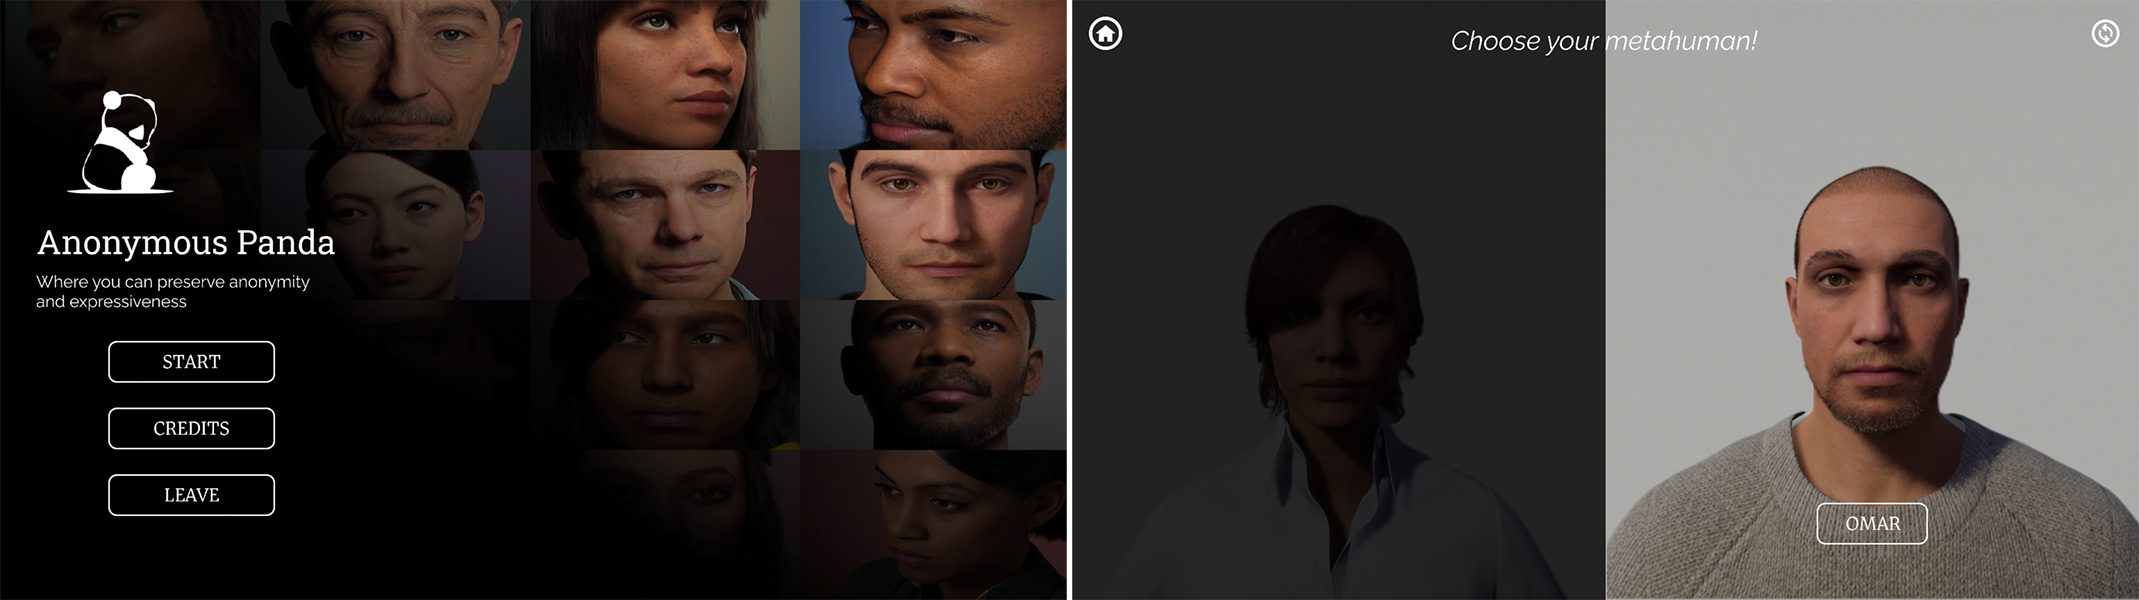
\includegraphics[width=\textwidth]{figures/ui-app.jpg}
\centering
\caption{Screenshots of the Anonymous Panda application}
\end{figure}

The human face is the primary means of non-verbal communication \cite{MALO20, KUJ03, SAU19}, used to communicate one's emotions and mood, and to provide visual cues of a person's physical state. Facial expressions are easily distinguished across cultures and automatically perceived so that we can immediately evaluate someone's emotional state. As Figure 5 makes visible, the facial expression of the VA are perceptible in the current version of the prototype. 

\begin{figure}[h!]
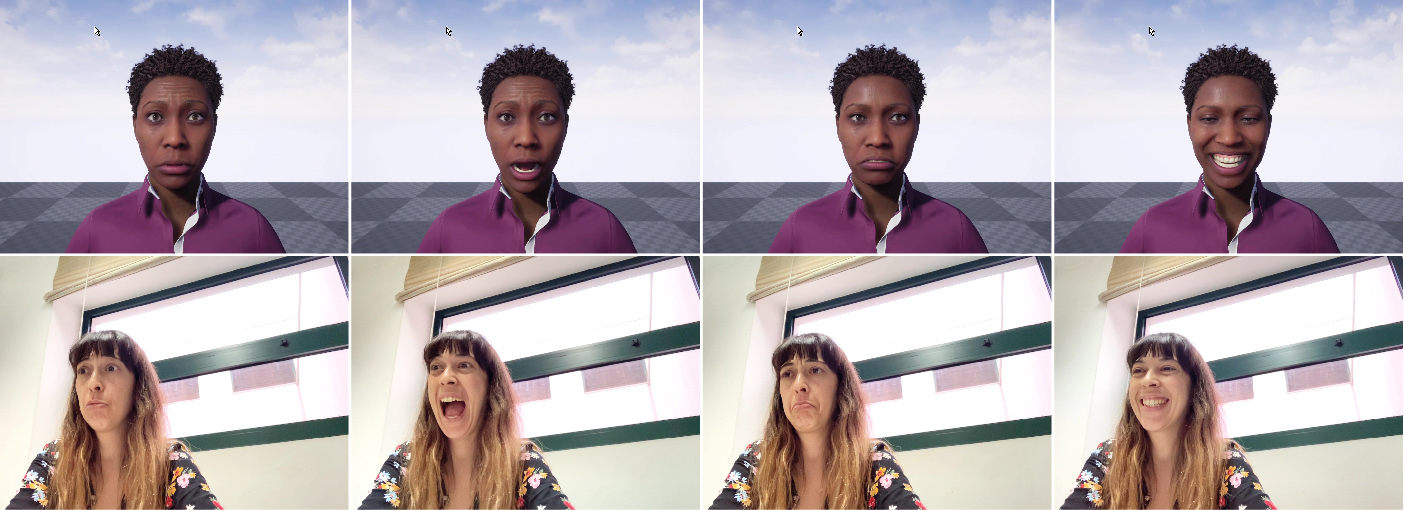
\includegraphics[width=\textwidth]{figures/expressionTest.jpg}
\centering
\caption{Examples of facial expressions and their virtual avatar depiction}
\end{figure}

However, upon a closer look, even though the avatar could accurately represent the user's facial expressions using the default functions of the live link plugin, a minor flaw in terms of lip positioning was found, particularly when the mouth should be closed or when the user was trying to express a negative emotion (e.g., sadness). To solve this issue, the upper lip values were slightly adjusted (Figure 6) before being reconverted to metahuman animation.

\begin{figure}[h!]
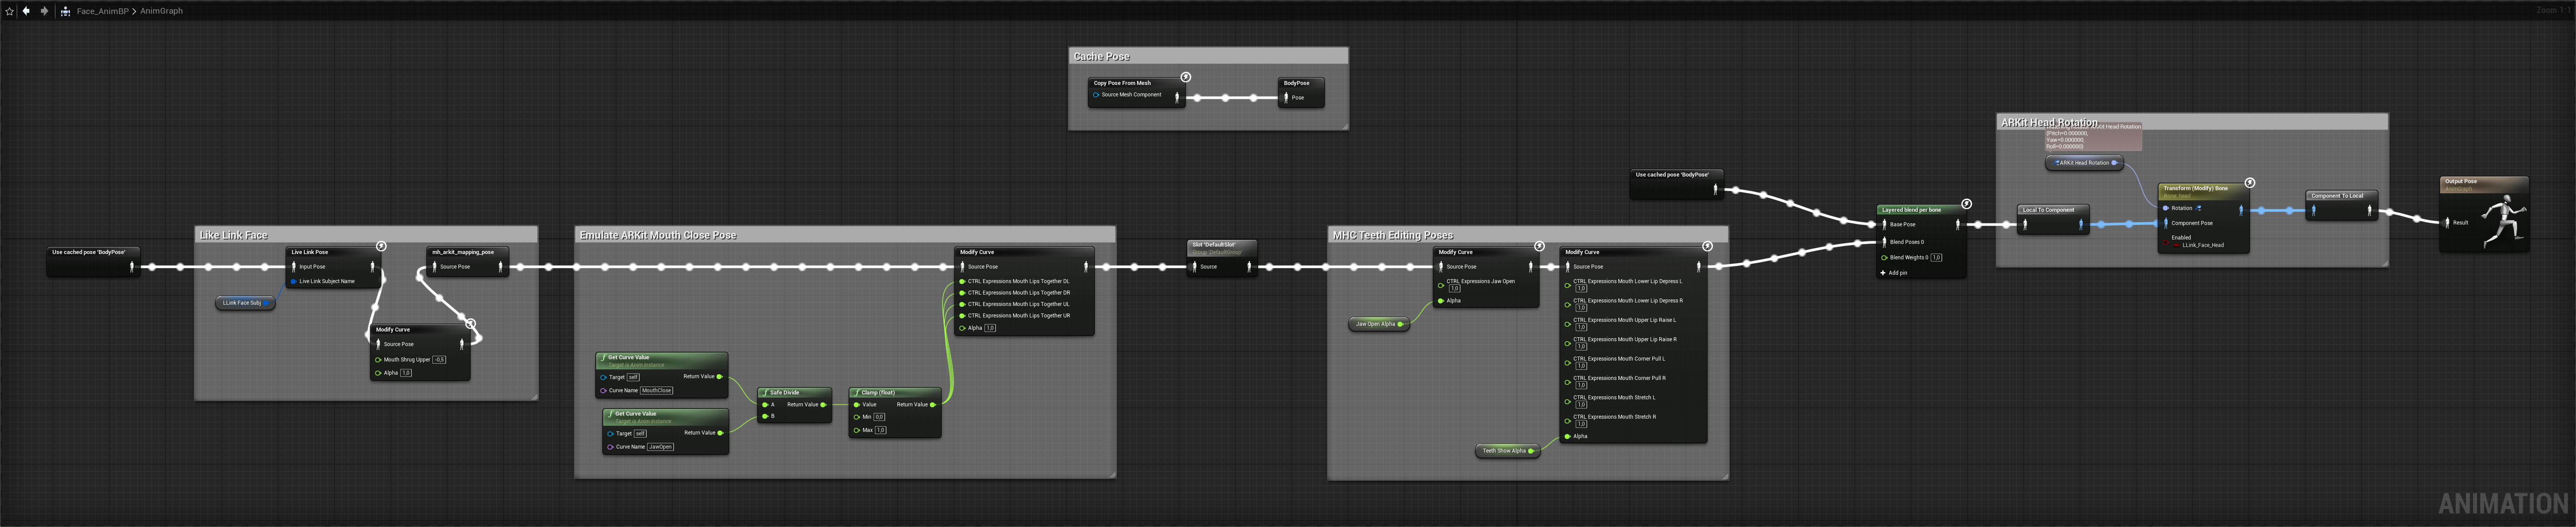
\includegraphics[width=\textwidth]{figures/facialConfig.png}
\centering
\caption{Blueprints responsible for the conversion of data to animation of metahuman}
\end{figure}

Although one of the foundations of this thesis is doctor-patient communication, the current prototype uses the UE4 application to emulate a webcam; meaning the user has to share their screen via a video conferencing tool (Figure 7). Even though this causes a slight delay, it can be used in a video conference.

\begin{figure}[h!]
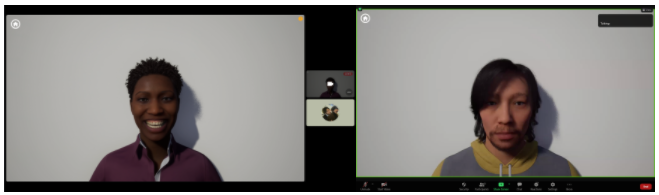
\includegraphics[width=\textwidth]{figures/zoomAndDiscord.PNG}
\centering
\caption{The prototype in use on a call via Discord and Zoom}
\end{figure}

\subsubsection{Limitations}
One of the thesis's challenges is to use customized models because these models demand a lot of optimization. After all, they are resource-intensive, limiting the patient's expressions from being viewed clearly and fluidly. 

Nonetheless, the creation and use of custom metahumans has already improved thanks to recent contributions from Epic Games. However, because many assets are still in development, the design and use of metahumans are still limited. That is, if these assets are excluded, it should be possible to use metahumans other than those pre-defined by Epic Games.

Finally, because this is a resource-intensive application, another difficulty is how people will utilize it. As a result, one of the problems is figuring out how to develop this program to reach everyone who needs it.

\subsection{Methodology}
To assess the feasibility of the previously described approach and test user's empathy with the metahumans, a controlled experiment will test whether this virtual avatars are able to convey the same emotional depth as a real person (RQ1).

\subsubsection{Procedure}
To do so, participants will be exposed to one of the following groups: a) pre-recorded metahuman, b) pre-recorded person, c) transcript from the previous pre-recorded contents (see Appendix A). The metahuman was created to match the appearance of the real person (Figure 8) as close as possible while keeping performance levels high (by using only optimized assets). This was done in order to avoid introducing excessive third-variable bias \cite{ROT19}, and the story was chosen from a specific \textit{subreddit} (i.e., an online community where people ask others for advice) based on the amount of \textit{upvotes} (1500) and number of comments (304) received on Reddit, as it provides a metric on user engagement and, therefore, we believe will help elicit empathy in the participants.

\begin{figure}[h!]
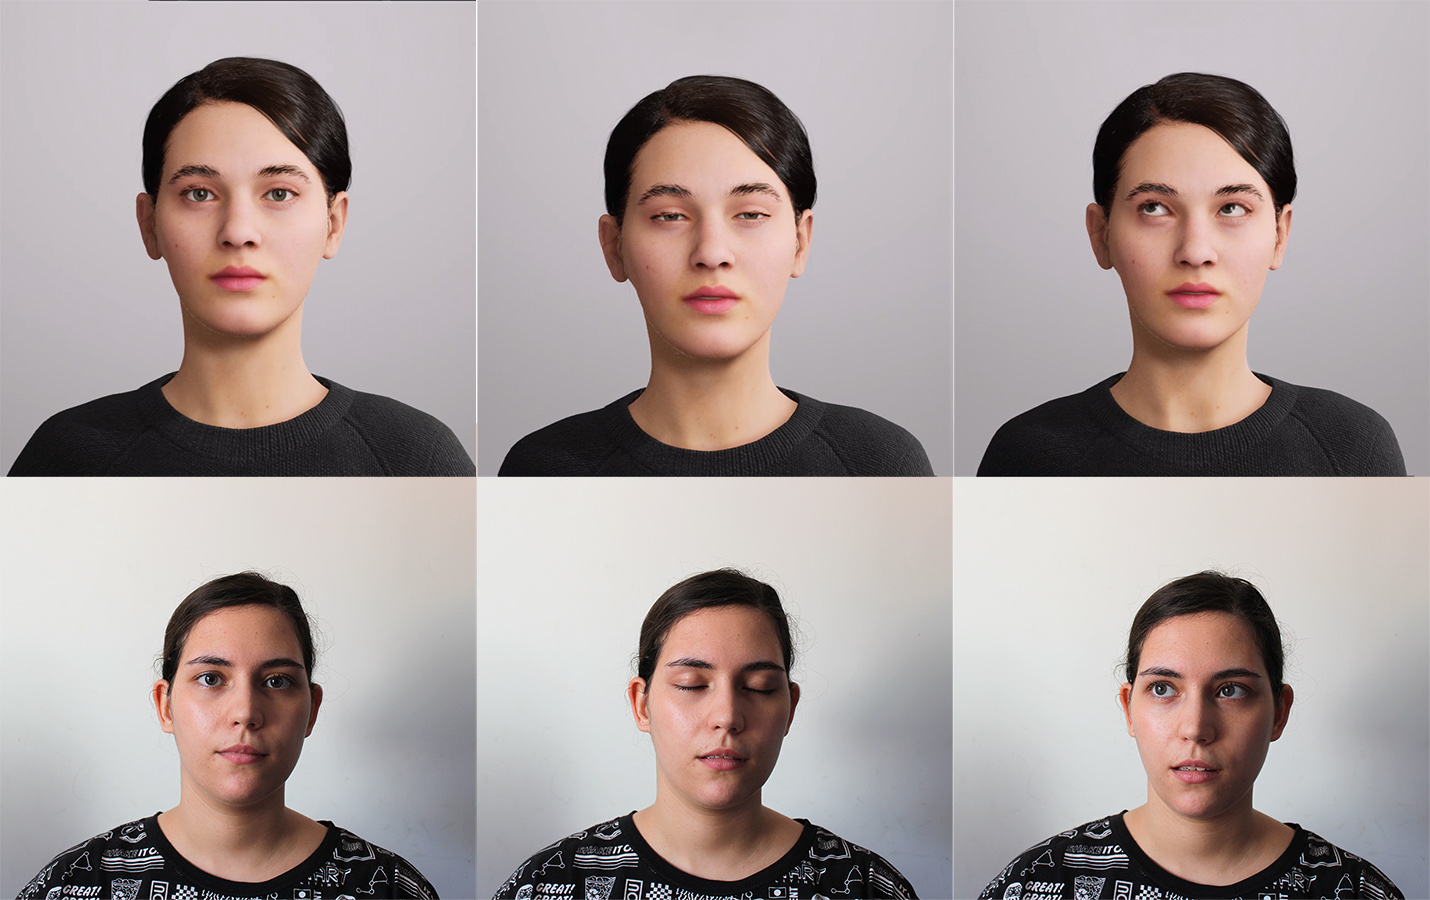
\includegraphics[width=\textwidth]{figures/personavatar.jpg}
\centering
\caption{Different expressions in both the custom metahuman and the actor}
\end{figure}

As it was not necessary to use the developed prototype in its entirety for this study, only the communication between the apple device and the Unreal Engine 4 for the metahuman's animation is required. As a result, the use of customized avatars has no effect on performance levels since all that is required to conduct this experiment is the capture of a local video from the UE4 application.

To avoid revealing the experiment's true purpose, and thus distorting the results, participants will be asked to answer some general questions about themselves (from the Big Five Inventory) in addition to the Toronto Empathy Questionnaire \cite{SPR03}, and the questionnaire developed to measure participants' empathy levels, as proposed by \cite{ROT19, ZIB19}. 
The experiment was accepted by the university's Data Protection Officer and authorized by the Ethics Committee and participants will be recruited via email, sent to the general student population from Madeira University, where they will be briefed about the study's broad, general topic.
The ones who agree to participate in the test will be asked to complete basic demographic questions and a personality questionnaire used to measure their baseline empathy levels prior to the video/transcript stimuli, and each participant will be randomly redirected to one of the three groups of content using \cite{FER19} and later asked some follow-up questions.

\subsubsection{Evaluation}
On the pre-test (Appendix B), the Toronto Empathy Questionnaire \cite{SPR03} will be utilized as a control variable, consisting of 16 items (e.g., "I become irritated when someone cries", 1=strongly disagree, to 5=strongly agree). To dispel any suspicions regarding the study's genuine goal, five items from the Big Five Inventory \cite{JOH91} will be incorporated into the questionnaire.

The dependent measures' questions will then be answered on a seven-point Likert-type scale (1=totally disagree, 7=totally agree) on the post-test (see Appendix C and D), based on the work of Bailenson et al. \cite{BAI03}.

We will use four questions to assess the video's perceived authenticity and social presence, presenting the statements ("I feel that the person is watching me and is aware of my presence", "The thought that the person is not a real person crosses my mind often", "The person appears to be conscious and alive to me", "I perceive the person as being only a computerized image, not as a real person") with the above-noted Likert-type scale.

Then, empathy will be tested in both video and transcript groups by using items adapted from the Interpersonal Reactivity Index \cite{DAV83} that deal with cognitive and affective empathy. Three items will be used to test cognitive empathy: "I understand what made her get upset", "Her reactions to the situation are understandable", and “I understand her point of view”. Afterwards three items will be used to measure emotional empathy ("I can relate to her problem", "When I see someone in an unfair situation, I feel frustrated", and “I feel that her emotions are genuine”).

Finally, participants can describe what made them empathize with and/or relate to the person in the video/transcript, as well as what they didn't like.

\subsubsection{Hypothesis}

\subsubsection{Participants}

\subsubsection{Results}
